\section{Thu, Mar 1st}
\subsection{Variance of the CP Problem}
Assuming a risk-averse central planner, we can compute the individual variance by
considering different cases
\begin{description}
\item[$x_i\in(0,\lambda_i=\frac{\lambda}{1-S_i\cdot UB})$]
In this case, the optimal rule corresponds to $r_i^*(x_i)=\lambda_i$ and the final expression of the variance does not depend on $x$. Nevertheless, it is given by
\[\var\{\pi_i(r^*_i(x_i)(1-\epsilon_i))\}=\displaystyle\begin{cases}
(a_1\lambda_i)^2\frac{(S_i\cdot UB)^2}{12}&1-\frac{\lambda}{\lambda_i}>S_i\cdot UB\\
0&1-\frac{\lambda}{\lambda_i}<0\\
\left(1-\frac{\lambda}{\lambda_i}\right)(a_1\lambda_i)^2\int_0^{1-\frac{\lambda}{\lambda_i}}(\tau-\Ex\epsilon)^2\Pro(d\tau)&{\rm o.w.}
\end{cases}\]

\item[$x_i\in(\lambda_i,\frac{a^0}{a^1}\frac{1}{1-\Ex\epsilon})$] Here, $r_i^*(x_i)=x_i$
\begin{eqnarray*}
\var\{\pi_i(r^*_i(x_i)(1-\epsilon_i))\}&=&\begin{cases}
(a_1 x)^2\frac{(S_i\cdot UB)^2}{12}&x\geq \lambda_i\\
\left(1-\frac{\lambda}{x}\right)^2\frac{(a_1\,x)^2}{3\,S_i\cdot UB}\left(\left(1-\frac{\lambda}{x}-\frac{S_i\cdot UB}{2}\right)^2-\frac{S_i\cdot UB}{2}\left(1-\frac{\lambda}{x}-\frac{S_i\cdot UB}{2}\right)+\left(\frac{S_i\cdot UB}{2}\right)^2\right)&{\rm o.w.}
\end{cases}
\end{eqnarray*}
\end{description}
\jd{check the regions!}

\subsection{Individual Variances}
The individual variance is given by
\begin{equation}\label{indvar}
\var\{\pi_i(r^*_i(x_i)(1-\epsilon_i))\}=\begin{cases}
(a_1\lambda_i)^2\frac{(S_i\cdot UB)^2}{12}&\lambda\leq x\leq \lambda_i\\
(a_1 x)^2\frac{(S_i\cdot UB)^2}{12}&\lambda_i\leq x\leq 1\\
0& {\rm ow}
\end{cases}
\end{equation}

\subsection{Pairwise Covariances}
Consider the nodes $i$ and $j$.  The covariance of the profits between these two institutions can be decompsed according to the values of $x_i$ and $x_j$.  It's easier to see this on the Figure~(\ref{figcovzones}).

\begin{figure}[htbp]
   \centering
   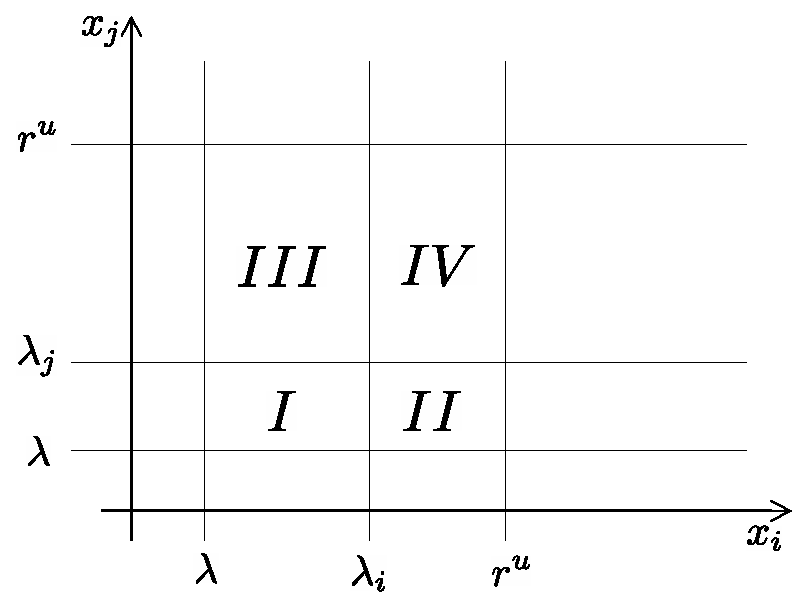
\includegraphics[width=0.5\textwidth]{CovAreas} % requires the graphicx package
   \caption{Areas for Covarianes}
   \label{figcovzones}
\end{figure}

After some algebra, the final form of the covariances is given by
\begin{equation}\label{eqcovij}
\cov(\pi_i(r^*_i(x_i(1-\epsilon_i))),\pi_j(r^*_j(x_j(1-\epsilon_j))))=\begin{cases}
(a_1)^2S_iS_j\lambda_i\lambda_j\frac{(UB)^2}{12}&\lambda\leq x_i\leq\lambda_i,\,\lambda\leq x_j\leq\lambda_j,(I)\\
(a_1)^2S_iS_j x_i\lambda_j\frac{(UB)^2}{12}&\lambda_i\leq x_i\leq r^u,\,\lambda\leq x_j\leq\lambda_j,(I)\\
(a_1)^2S_iS_j \lambda_i x_j\frac{(UB)^2}{12}&\lambda\leq x_i\leq \lambda,\,\lambda_j\leq x_j\leq r^u,(III)\\
(a_1)^2S_iS_j x_i x_j\frac{(UB)^2}{12}&\lambda_i\leq x_i \leq r^u \lambda,\,\lambda_j\leq x_j\leq r^u,(IV)\\
0&{\rm ow}
\end{cases}
\end{equation}